\documentclass[11pt,a4paper]{article}
\usepackage[russian]{babel}
\usepackage[utf8]{inputenc}
\usepackage{amsmath}
\usepackage{mathtools} 
\usepackage{amssymb}
\usepackage{multicol}
\usepackage{bm}
\usepackage[hcentering, bindingoffset = 10mm, right = 15 mm, left = 15 mm, top=20mm, bottom = 20 mm]{geometry}
\newcounter{prim}
\newenvironment{prim}{%
	\addtocounter{prim}{1}
	\noindent{\\
		\textbf{\noindentПример \arabic{prim}\\}}%
}{}

\DeclareMathOperator{\tr}{\mathop{tr}}
\DeclareMathOperator{\Ker}{\mathop{Ker}}
\DeclareMathOperator{\im}{\mathop{Im}}
\DeclareMathOperator{\const}{\mathop{const}}
\DeclareMathOperator{\rg}{\mathop{rg}}
\newtheorem{definition}{Определение}[section]
\newtheorem{theorem}{Теорема}[section]
\renewcommand{\labelenumi}{\asbuk{enumi})}

\begin{document}
	\part*{Лабораторная работа 3.3.3}
	\part*{Опыт Милликена}
	\textbf{Работу выполнили:} \\
	{\itshape Морозов Матвей \\ Бабушкина Татьяна \\ 678 группа} \\\\
\textbf{Цель работы:} измерение элементарного заряда методом масляных капель.
\\\\
\textbf {В работе используются:} плоский конденсатор в защитном кожухе, осветитель, измерительный микроскоп, электостатический  вольтметр, электронный секндомер, переключатель напряжения, пульверизатор с маслом.
\\
\\
\part*{Теоретические выкладки}

Если елементарный заряд действительно существует, то заряд $q$ любого тела может принимать только дискретную последовательность значений:\\
\begin{center}
$q = 0, \pm e, \pm 2e, \pm 3e, \cdots, \pm ne$
\end{center}
В предлагаемом опыте измеряется заряд небольших капелек масла, несущих всего несколько элементарных зарядов. Сравивая между собой заряды капель, можно убедиться, что все они по модулю кратны одному и тому же числу, которое равно, очевидно, элментарному заряду - $e$.\\
Рассмотрим свободное падение капли. Уравнение движения при падении примет вид: \\
\begin{center}
$m \cfrac{dv}{dt} = mg -F$, 
\end{center}
где $F$ - сила вязкого трения капли в воздухе, которая для сферической капли определяется формулой Стокса:\\
\begin{center}
$F = 6 \pi \eta r v = kv$
\end{center}
Здесь $r$ - радиус капли, $\eta$ - коэффициент вязкости воздуха, $k = 6 \pi \eta r$\\
Теперь получим:\\
\begin{center}
$ь \cfrac{dv}{dt} = mg - kv$
\end{center}
Можно убедиться, что при нулевой начально скорости решение этого уравнения имеет  вид:\\
\begin{center}
$v = \cfrac{mg}{k} (1 - e^{- \frac{kt}{m}})$
\end{center}
Установившееся значение скорости равно:\\
\begin{center}
$v_0 = \cfrac{mg}{k} = \cfrac{\frac{4}{3} \pi p r^3 g}{6 \pi \eta r} = \cfrac{2 p g r^2}{9 \eta}$,
\end{center}
где $p$ - плотность масла.
\\
Заметим, что при $\cfrac{dv}{dt} = 0$ следует установление скорости с постоянной времени $\tau$:\\
\begin{center}
$\tau = \cfrac{m}{k} = \cfrac{2 p r^2}{9 \eta}$
\end{center}
Время установления скорости быстро падает с уменьшением радиуса капли. Для очень маленьких капель оно столь мало, что движение капли можно счиать равномерным.\\
Обозначая через $h$ путь, пройденный каплей за время $t_0$, найдем:\\
\begin{center}
$r = \sqrt{\cfrac{9 \eta h}{2 p g t_0}}$.
\end{center}
При подъеме капли уравнение движения примет вид:\\
\begin{center}
$ь \cfrac{dv}{dt} = \cfrac{qV}{l} - mg - kv$, 
\end{center}
где $E = \cfrac{V}{l}$, $q$ - заряд капли.\\
Измерим время $t$ подъема капли на начальную высоту. Использую предыдущие уравнения, найдем:
\begin{center}
$q = 9 \pi \sqrt{\cfrac{2 \eta^3 h^3}{g p}} \cfrac{l(t + t_0)}{V {t_0}^{\frac{3}{2}}t}$
\end{center}
\part*{Экспериментальная установка}
\begin{figure}[h!]
	\centering
	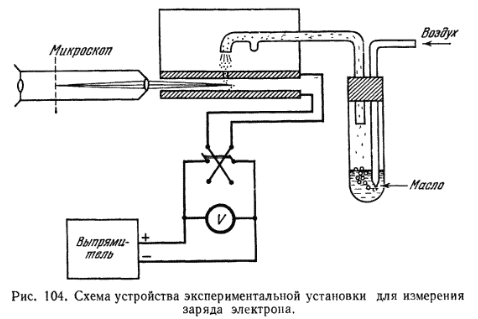
\includegraphics[width=0.6\linewidth]{exp}
\end{figure}
Напряжение на пластины подается с регулируемого выпрямителя и измеряется вольтметром $V$. Ключ $K$ позволяет менять поля в конденсаторе, чтобы было можно работать как с отрицательно, так и с положительно заряженными каплями. При размыкании конденсатор разряжается через дополнительное сопротивление.\\
Время отсчитывается по элетронному секундомеру.\\
\newpage
Из всех величин в формулу для заряда, на опыте измеряются только $t_0, t, V$. От точности этих величин зависит в соновном ошибка измерения $q$.\\
\begin{center}
$ \cfrac{\sigma_q}{q} = \sqrt{\cfrac{\sigma_V^2}{V^2} + \cfrac{\sigma_t^2 t_0^2}{t^2(t_0 + t)^2} + \cfrac{\sigma_{{t_0}^2}}{4t_0^2}({\cfrac{3t +t_0}{t + t_0}})^2}$
\end{center}
При $t_0 \approx t$ формула приобретет вид:\\
\begin{center}
$\cfrac{\sigma_q}{q} = \sqrt{ \cfrac{\sigma_V^2}{V^2}} + \cfrac{\sigma_t^2}{4t_0^2} + \cfrac{\sigma_{t_0}^2}{t_0^2}$
\end{center}
В условиях нашей работы наибольшее влияние на точность эксперимента оказывают два последних стоящих под корнем члена. ошибка измерения времени при визуальном наблюдении капель не может быть меньше $0,1 - 0,2$ секунды. То есть погрешность будет принимать меньшие значения при измерении больших $t$ и $t_0$.
\part*{Измерения и вычисления}
\begin{table}[h!]
	\begin{center}
		\textbf{Таблица 1}. Зависимость $t$ и $t_0$ от $U$ для капли $№1$.\\
	\begin{tabular}{|c|c|c|c|c|c|c|c|c|c|}
		
			\hline
			 & \textbf{1} & \textbf{2} & \textbf{3} &\textbf{4} &\textbf{5} & СР З & $\sigma$ & q& $\sigma q$\\ \hline
			$U$, В & 200 & 200 & 200 & 200 & 200 &  200 &  1 \\ \hline
			$t_0$, c  & 33,84 & 31,25 & 32,75 & 32,64 & 31,95&  32,486 & 0,748 & 1,1696E-19
& 7,90524E-21
\\ \hline
			$t$, c   & 17,81 & 17,69 & 17,84 & 17,45 & 17,93 & 17,744 & 0,027 \\ \hline
	\end{tabular}
	\end{center}
\end{table}
\space
\begin{table}[h!]
	\begin{center}
		\textbf{Таблица 2}. Зависимость $t$ и $t_0$ от $U$ для капли $№2$.\\
	\begin{tabular}{|c|c|c|c|c|c|c|c|c|c|}
		
			\hline
			 & \textbf{1} & \textbf{2} & \textbf{3} &\textbf{4} &\textbf{5} & СР З & $\sigma$  & q& $\sigma q$  \\ \hline
			$U$, В & 260 & 260 & 260 & 260 & 260 &  260 &  1 \\ \hline
			$t_0$, c  & 32,89 & 29,51 & 31,76 & 34,42 & 32,27& 32,17  & 2,566 & 1,46145E-19
& 2,23906E-21
\\ \hline
			$t$, c   & 13,36 & 13,14 & 12,48 & 13,53 & 12,20 & 12,942 & 0,264 \\ \hline
	\end{tabular}
	\end{center}
\end{table}
\space
\begin{table}
	\begin{center}
		\textbf{Таблица 3}. Зависимость $t$ и $t_0$ от $U$ для капли $№3$.\\
	\begin{tabular}{|c|c|c|c|c|c|c|c|c|c|}
		
			\hline
			 & \textbf{1} & \textbf{2} & \textbf{3} &\textbf{4} &\textbf{5} & СР З & $\sigma$  & q& $\sigma q$ \\ \hline
			$U$, В & 300 & 300 & 300 & 300 & 300 &  300 &  1 \\ \hline
			$t_0$, c  & 27,16 & 27,09 & 26,23 & 26,74 & 27,05&  26,854 & 0,118 & 1,6629E-19
 & 2,29207E-20
 \\ \hline
			$t$, c   & 13,09 & 13,82 & 11,79 & 14,25 & 13,36 & 13,262 & 0,698 \\ \hline
	\end{tabular}
	\end{center}
\end{table}
\space
\begin{table}
	\begin{center}
		\textbf{Таблица 4}. Зависимость $t$ и $t_0$ от $U$ для капли $№4$.\\
	\begin{tabular}{|c|c|c|c|c|c|c|c|c|c|}
		
			\hline
			 & \textbf{1} & \textbf{2} & \textbf{3} &\textbf{4} &\textbf{5} & СР З & $\sigma$  & q& $\sigma q$  \\ \hline
			$U$, В & 340 & 340 & 340 & 340 & 340 &  340 &  1 \\ \hline
			$t_0$, c  & 35,05  & 40,29 & 36,93 & 40,23 & 36,74 & 37,848  & 4,307 & 1,8729E-19
 & 3,68434E-21
\\ \hline
			$t$, c   & 8,07 & 8,81 & 7,69 & 7,74 & 7,95 & 8,052 & 0,162\\ \hline
	\end{tabular}
	\end{center}
\end{table}
\space\begin{table}
	\begin{center}
		\textbf{Таблица 5}. Зависимость $t$ и $t_0$ от $U$ для капли $№5$.\\
	\begin{tabular}{|c|c|c|c|c|c|c|c|c|c|}
		
			\hline
			 & \textbf{1} & \textbf{2} & \textbf{3} &\textbf{4} &\textbf{5} & СР З & $\sigma$  & q& $\sigma q$ \\ \hline
			$U$, В & 400 & 400 & 400 & 400 & 400 &  400 &  1 \\ \hline
			$t_0$, c  & 32,52 & 30,98 & 33,04 & 31,75 & 32,79 &  32,216 & 0,569 & 2,0237E-19
 & 1,48523E-20
\\ \hline
			$t$, c   & 7,81 & 8,34 & 9,07 & 8,07 & 8,69 & 8,396 & 0,198 \\ \hline
	\end{tabular}
	\end{center}
\end{table}

\begin{table}
	\begin{center}
		\textbf{Таблица 6}. Зависимость $t$ и $t_0$ от $U$ для капли $№6$.\\
	\begin{tabular}{|c|c|c|c|c|c|c|c|c|c|}
		
			\hline
			 & \textbf{1} & \textbf{2} & \textbf{3} &\textbf{4} &\textbf{5} & СР З & $\sigma$  & q& $\sigma q$ \\ \hline
			$U$, В & 460 & 460 & 460 & 460 & 460 &  460 & 1  \\ \hline
			$t_0$, c  & 31,18 & 26,62 & 26,42 & 29,23 & 27,45 &  28,18 & 3,233 & 3,39595E-19
 & 4,69271E-20
\\ \hline
			$t$, c   & 4,47 & 5,13 & 5,5 & 5,23 & 4,65 & 4,996 & 0,144\\ \hline
	\end{tabular}
	\end{center}
\end{table}
\space\begin{table}
	\begin{center}
		\textbf{Таблица 7}. Зависимость $t$ и $t_0$ от $U$ для капли $№7$.\\
	\begin{tabular}{|c|c|c|c|c|c|c|c|c|c|}
		
			\hline
			 & \textbf{1} & \textbf{2} & \textbf{3} &\textbf{4} &\textbf{5} & СР З & $\sigma$  & q& $\sigma q$ \\ \hline
			$U$, В & 520 & 520 & 520 & 520 & 520 &  520 & 1  \\ \hline
			$t_0$, c  & 35,63 & 33,69 & 28,94 & 32,9 & 30,09 &  32,244 & 5,890 & 2,82362E-19
 & 4,9673E-21
\\ \hline
			$t$, c   & 5,95 & 5,83 & 5,33 & 5,67 & 5,22 & 5,600 & 0,079\\ \hline
	\end{tabular}
	\end{center}
\end{table}
\space\begin{table}
	\begin{center}
		\textbf{Таблица 8}. Зависимость $t$ и $t_0$ от $U$ для капли $№8$.\\
	\begin{tabular}{|c|c|c|c|c|c|c|c|c|c|}
		
			\hline
			 & \textbf{1} & \textbf{2} & \textbf{3} &\textbf{4} &\textbf{5} & СР З & $\sigma$  & q& $\sigma q$ \\ \hline
			$U$, В & 580 & 580 & 580 & 580 & 580 &  580 &  1 \\ \hline
			$t_0$, c  & 23,28 & 24,39 & 22,10 & 23,31 & 22,45 &  23,106 & 0,632 & 2,98732E-19
 & 5,1494E-21
\\ \hline
			$t$, c   & 6,88 & 7,01 & 6,64 & 6,24 & 7,85 & 6,924 & 0,283 \\ \hline
	\end{tabular}
	\end{center}
\end{table}
\space\begin{table}
	\begin{center}
		\textbf{Таблица 9}. Зависимость $t$ и $t_0$ от $U$ для капли $№9$.\\
	\begin{tabular}{|c|c|c|c|c|c|c|c|c|c|}
		
			\hline
			 & \textbf{1} & \textbf{2} & \textbf{3} &\textbf{4} &\textbf{5} & СР З & $\sigma$  & q& $\sigma q$ \\ \hline
			$U$, В & 640 & 640 & 640 & 640 & 640 &  640 &  1 \\ \hline
			$t_0$, c  & 37,95 & 44,06 & 40,02 & 38,38 & 42,21 & 40,524  & 5,360 & 1,46603E-19
 & 6,59035E-21
\\ \hline
			$t$, c   & 11,49 & 10,58 & 9,43 & 9,77 & 10,11 & 10,276 & 0,513\\ \hline
	\end{tabular}
	\end{center}
\end{table}
\space\begin{table}
	\begin{center}
		\textbf{Таблица 10}. Зависимость $t$ и $t_0$ от $U$ для капли $№10$.\\
	\begin{tabular}{|c|c|c|c|c|c|c|c|c|c|}
		
			\hline
			 & \textbf{1} & \textbf{2} & \textbf{3} &\textbf{4} &\textbf{5} & СР З & $\sigma$  & q& $\sigma q$  \\ \hline
			$U$, В & 520 & 520 & 520 & 520 & 520 &  520 &  1 \\ \hline
			$t_0$, c  & 27,72 & 29,96 & 26,77 & 28,45 & 27,38 & 28,056  & 1,200 &2,49492E-19
 & 3,64036E-21
\\ \hline
			$t$, c   & 9,69 & 6,03 & 6,63 & 7,45 & 6,67 & 7,294 & 1,280 \\ \hline
	\end{tabular}
	\end{center}
\end{table}
\space\begin{table}
	\begin{center}
		\textbf{Таблица 11}. Зависимость $t$ и $t_0$ от $U$ для капли $№11$.\\
	\begin{tabular}{|c|c|c|c|c|c|c|c|c|c|}
		
			\hline
			 & \textbf{1} & \textbf{2} & \textbf{3} &\textbf{4} &\textbf{5} & СР З & $\sigma$  & q& $\sigma q$ \\ \hline
			$U$, В & 520 & 520 & 520 & 520 & 520 &  520 &  1 \\ \hline
			$t_0$, c  & 18,72 & 17,72 & 21,68 & 19,21 & 18,93 & 19,252  & 1,726 & 2,94297E-19
			& 9,97962E-21
\\ \hline
			$t$, c   & 8,56 & 9,3 & 8,77 & 7,95 & 8,21 & 8,558 & 0,217\\ \hline
	\end{tabular}
	\end{center}
\end{table}
\begin{table}
	\begin{center}
		\textbf{Таблица 12}. Зависимость $t$ и $t_0$ от $U$ для капли $№12$.\\
	\begin{tabular}{|c|c|c|c|c|c|c|c|c|c|}
		
			\hline
			 & \textbf{1} & \textbf{2} & \textbf{3} &\textbf{4} &\textbf{5} & СР З & $\sigma$ & q& $\sigma q$  \\ \hline
			$U$, В & 520 & 520 & 520 & 520 & 520 &  520 & 1  \\ \hline
			$t_0$, c  & 29,57 & 31,23 & 30,59 & 28,9 & 29,55 &  29,968 & 0,690 & 2,78615E-19
 & 3,00662E-21
\\ \hline
			$t$, c   & 5,67 & 6,21 & 6,01 & 6,25 & 5,98 & 6,024 & 0,042 \\ \hline
	\end{tabular}
	\end{center}
\end{table}
\begin{table}
	\begin{center}
		\textbf{Таблица 13}. Зависимость $t$ и $t_0$ от $U$ для капли $№13$.\\
	\begin{tabular}{|c|c|c|c|c|c|c|c|c|c|}
		
			\hline
			 & \textbf{1} & \textbf{2} & \textbf{3} &\textbf{4} &\textbf{5} & СР З & $\sigma$  & q& $\sigma q$ \\ \hline
			$U$, В & 520 & 520 & 520 & 520 & 520 &  520 &  1 \\ \hline
			$t_0$, c  & 37,92 & 34,02 & 27,98 & 24,61 & 27,57 & 30,42  & 4,838 & 2,95695E-19
 & 2,16417E-21
\\ \hline
			$t$, c   & 5,38 & 5,51 & 5,50 & 5,60 & 5,74 & 5,546 & 0,014 \\ \hline
	\end{tabular}
	\end{center}
\end{table}
\begin{table}[h!]
	\begin{center}
		\textbf{Таблица 14}. Зависимость $t$ и $t_0$ от $U$ для капли $№14$.\\
	\begin{tabular}{|c|c|c|c|c|c|c|c|c|c|}
		
			\hline
			 & \textbf{1} & \textbf{2} & \textbf{3} &\textbf{4} &\textbf{5} & СР З & $\sigma$  & q& $\sigma q$ \\ \hline
			$U$, В & 520 & 520 & 520 & 520 & 520 &  520 & 1  \\ \hline
			$t_0$, c  & 31,37 & 31,46 & 29,93 & 30,93 & 30,58 & 30,854  & 0,313 & 2,92346E-19
 & 1,70206E-21
\\ \hline
			$t$, c   & 5,83 & 5,43 & 5,38 & 5,51 & 5,65 & 5,560 & 0,026 \\ \hline
	\end{tabular}
	\end{center}
\end{table}
\begin{table}[h!]
	\begin{center}
		\textbf{Таблица 15}. Зависимость $t$ и $t_0$ от $U$ для капли $№15$.\\
	\begin{tabular}{|c|c|c|c|c|c|c|c|c|c|}
		
			\hline
			 & \textbf{1} & \textbf{2} & \textbf{3} &\textbf{4} &\textbf{5} & СР З & $\sigma$  & q& $\sigma q$ \\ \hline
			$U$, В & 520 & 520 & 520 & 520 & 520 &  520 & 1  \\ \hline
			$t_0$, c  & 23,71 & 22,54 & 23,44 & 22,79 & 23,02 & 23,100  & 0,180 & 3,10293E-19
 & 2,06489E-21
\\ \hline
			$t$, c   & 6,53 & 6,62 & 5,98 & 6,25 & 6,59 & 6,594 & 0,054\\ \hline
	\end{tabular}
	\end{center}
\end{table}
\newpage
\part*{Обработка результатов}
1)Для всех исследованных капель расситайте значения $q$, отложим их на горизонтальной числовой оси и найдите для них общий наибольший делитель. Этот наибольший делитель, вообще говоря, может оказаться равным $e, 2e, 3e$ и тд.
\begin{figure} [h!]
	\centering
	\textbf {График 1} \\
	Полученные значения q на оси\\
	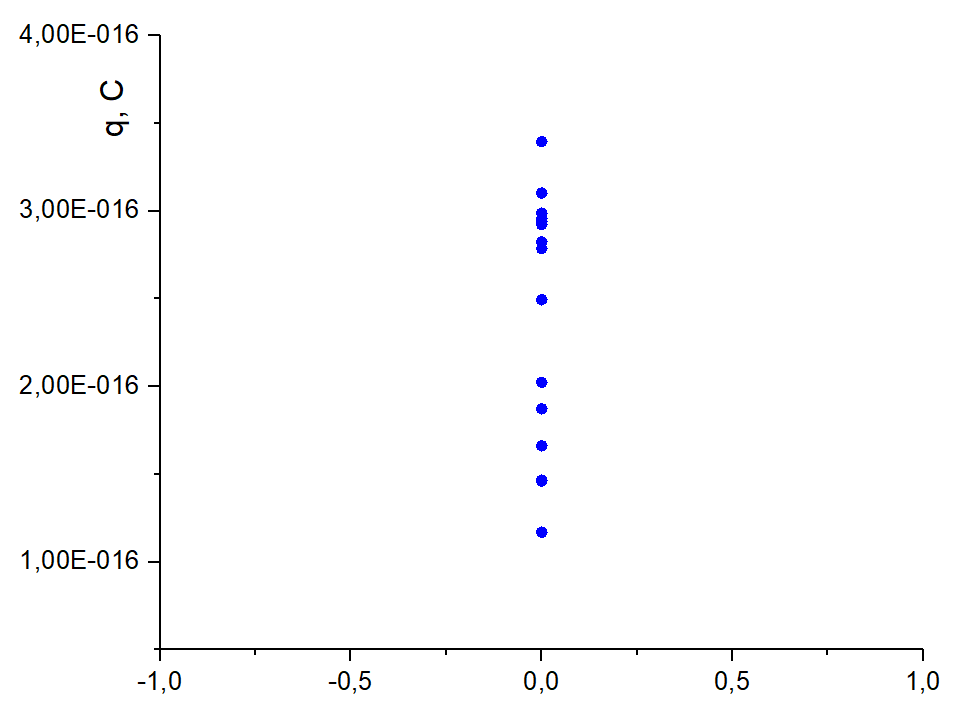
\includegraphics[width=0.5\linewidth]{1.png}
\end{figure}
\newpage

2)Теперь оценим время релаксации $ \tau = \cfrac{v_{o}}{g}$ и $s = \cfrac{h^2}{gt_0^2}$ - расстояние, которое капля прошла за это время с установившейся скоростью.\\
Установившееся значение скорости равно:\\
\begin{center}
$v_0 = \cfrac{mg}{k} = \cfrac{\frac{4}{3} \pi p r^3 g}{6 \pi \eta r} = \cfrac{2 p g r^2}{9 \eta}$,
\end{center}
где $p$ - плотность масла, а $r = \sqrt{\cfrac{9 \eta h}{2 p g t_0}}$ \\
Следовательно, $v_0 = \cfrac{h}{t_0}$, $\tau = \cfrac{h}{gt_0}$:\\

\begin{table}[h!]
	\begin{center}
\textbf{Таблица 16}.\\
\begin{tabular}{|c|c|}
\hline
$\tau, 10^{-6} \cdot \text{с}$ & $s, 10^{-11} \cdot \text{м}$ \\ \hline
3,141 &	9,669 \\ \hline
3,172 & 14,150 \\ \hline
2,696 &	7,123 \\ \hline
3,167 &	9,832 \\ \hline
3,621 &	12,850 \\ \hline
3,165 &	9,815 \\ \hline
4,416 &	19,113 \\ \hline
2,518 &	6,214 \\ \hline
3,637 &	12,964 \\ \hline
5,300 &	27,531 \\ \hline
3,405 & 11,362 \\ \hline
3,354 &	11,027 \\ \hline
3,307 &	10,719 \\ \hline
4,416 &	19,123 \\ \hline
	\end{tabular}
	\end{center}
\end{table}


\part*{Вывод}
В ходе лабораторной работы:
\begin{enumerate}
	\item 
	Посчитали заряд электрона. \\ Из графика $1$ видно, что заряды молекул масла распределились около значений $1,5 \cdot 10^{-19} \ \ \text{Кл}$ и $3 \cdot 10^{-19} \ \ \text{Кл}$.
Таким образом, заряд электрона примерно равен $1,5 \cdot 10^{-19} \ \ \text{Кл} = 4,5 \cdot 10^{-9} \ \ \text{Фр}$.
\item Оценили время релаксации и расстояние, которое прошла бы капля с установившейся скоростью (см. таблицу $16$).
\end{enumerate}
\end{document}